\documentclass[10pt]{article}

\usepackage[margin=1in]{geometry}
\usepackage{amsmath,amssymb,amsthm}
\usepackage{booktabs}
\usepackage{graphicx}
\usepackage{microtype}
\usepackage{enumitem}
\usepackage{tikz}
\usepackage{hyperref}
\usepackage[numbers,sort&compress]{natbib}
\usetikzlibrary{arrows.meta,positioning}

\title{Stochastic Transitive Reinforcement Learning:\\
Calibrated Divide-and-Conquer Value Propagation under Stochastic Dynamics}
\author{Anonymous Authors}
\date{}

\newtheorem{theorem}{Theorem}
\newtheorem{proposition}{Proposition}
\newtheorem{assumption}{Assumption}

\newcommand{\states}{\mathcal{S}}
\newcommand{\actions}{\mathcal{A}}
\newcommand{\E}{\mathbb{E}}
\newcommand{\Phat}{\widehat{P}}
\newcommand{\one}{\mathbf{1}}

\begin{document}
\maketitle

\begin{abstract}
Long-horizon offline goal-conditioned reinforcement learning requires
propagating sparse reachability information across many decision steps.
Transitive RL (TRL) shows that deterministic goal-reaching problems contain a
divide-and-conquer structure: if an agent can reach an intermediate subgoal
and then reach the final goal, long paths can be propagated in logarithmically
many transitive sweeps. This deterministic composition is not calibrated in
stochastic environments. A lucky rollout through a risky shortcut or teleporter
is only one outcome from a transition distribution, but deterministic
realized-path composition can treat it as a reliable edge. We introduce
\emph{Stochastic Transitive RL}, a calibrated transitive value-iteration
algorithm that composes stochastic reachability probabilities instead of
binary realized path labels. Each update combines an empirical Bellman
expectation backup, which calibrates stochastic outcomes, with a transitive
product backup, which propagates reliable long-horizon reachability. In
tabular stochastic shortcut tasks and 2D stochastic grid shortcuts, Stochastic
TRL learns safe long-horizon policies with logarithmic matched sweep budgets,
where matched Bellman and realized-positive baselines choose risky shortcuts.
On OGBench PointMaze teleport navigate and stitch diagnostics, Stochastic TRL
reaches 0.901 mean success with a 6-sweep budget, matching a 180-sweep Bellman
reference while matched Bellman reaches 0.343. On OGBench AntMaze teleport
with learned BC executors, Stochastic TRL reaches 0.947 success on navigate
and 0.960 on stitch, again matching the long-sweep Bellman reference while
matched Bellman remains near 0.31. Across three independently trained AntMaze
controllers for each task, Stochastic TRL remains above 0.933 success on
navigate and above 0.950 success on stitch. In a learned high-level module
screen that replaces both table transition fitting and table action values
with raw-observation MLP heads, Stochastic TRL still reaches 0.933 success on
AntMaze navigate and 0.967 on AntMaze stitch across three evaluation seeds.
A controlled learned-critic screen further shows that a small MLP trained with
the stochastic transitive target solves all safe-optimal stochastic shortcut
settings, while matched neural Bellman and support-only transitive critics fail.
\end{abstract}

\section{Introduction}

Goal-conditioned reinforcement learning (GCRL) asks an agent to reach arbitrary
goal states. In the offline setting, this problem is particularly sensitive to
long-horizon value propagation: a Bellman backup transmits sparse reachability
information one transition at a time, so a path of length $H$ requires roughly
$H$ value-iteration sweeps before the start state sees the goal. Transitive RL
\citep{park2026transitive} addresses this in deterministic environments by
turning a triangle-inequality structure into a divide-and-conquer value update.
If a policy can reach $w$ from $s$ and then reach $g$ from $w$, a transitive
backup can compose these two shorter subproblems and propagate length-$H$
structure in $O(\log H)$ sweeps.

The same idea is not directly valid in stochastic environments. A successful
trajectory segment through a stochastic teleporter or risky shortcut is not a
reliable transition; it is one sampled outcome from a transition distribution.
Composing such samples as if they were deterministic edges creates optimistic
plans that exploit lucky outcomes. This failure mode is directly relevant to
modern offline GCRL benchmarks such as OGBench, whose tasks include
long-horizon stitching and stochastic teleport dynamics \citep{park2024ogbench}.

This paper studies that tension and proposes Stochastic Transitive RL. The
central change is simple: compose calibrated stochastic reachability estimates,
not realized path labels. The resulting operator uses a Bellman expectation
backup to estimate the probability of reaching subgoals under stochastic
dynamics, and a transitive product backup to propagate long-horizon routes.
The Bellman term keeps stochastic shortcuts calibrated; the transitive term
keeps TRL's horizon efficiency on reliable paths.

\begin{figure}[t]
\centering
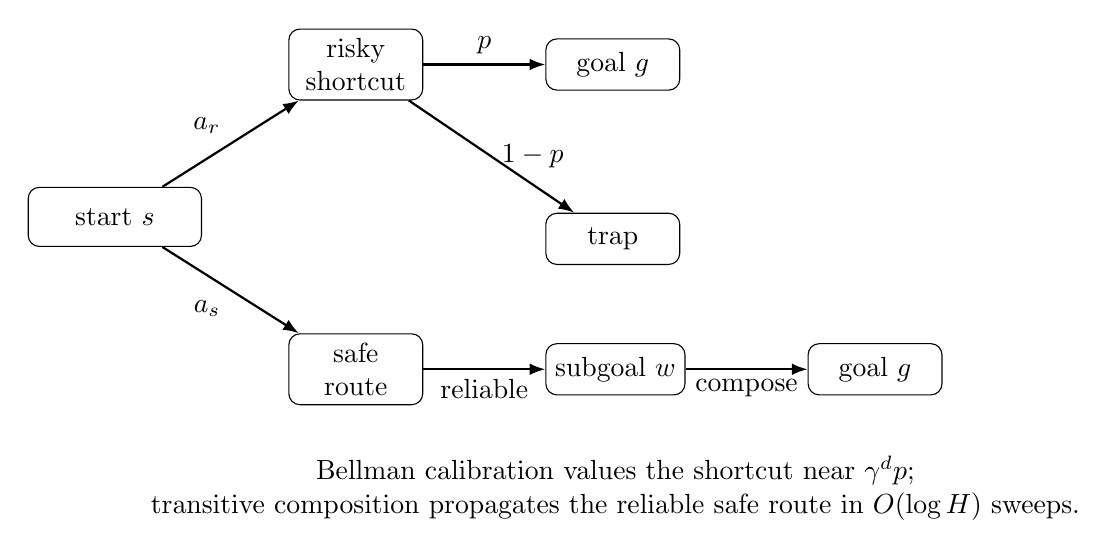
\begin{tikzpicture}[
    node distance=1.55cm,
    box/.style={draw, rounded corners, align=center, minimum width=2.2cm, minimum height=0.75cm},
    smallbox/.style={draw, rounded corners, align=center, minimum width=1.7cm, minimum height=0.65cm},
    arr/.style={-{Latex[length=2mm]}, thick}
]
\node[box] (start) {start $s$};
\node[smallbox, above right=of start] (risky) {risky\\shortcut};
\node[smallbox, right=of risky] (goal1) {goal $g$};
\node[smallbox, below=of goal1] (trap) {trap};
\node[smallbox, below right=of start] (safe1) {safe\\route};
\node[smallbox, right=of safe1] (mid) {subgoal $w$};
\node[smallbox, right=of mid] (goal2) {goal $g$};
\draw[arr] (start) -- node[above left] {$a_r$} (risky);
\draw[arr] (risky) -- node[above] {$p$} (goal1);
\draw[arr] (risky) -- node[right] {$1-p$} (trap);
\draw[arr] (start) -- node[below left] {$a_s$} (safe1);
\draw[arr] (safe1) -- node[below] {reliable} (mid);
\draw[arr] (mid) -- node[below] {compose} (goal2);
\node[align=center, below=0.65cm of mid] {
Bellman calibration values the shortcut near $\gamma^d p$;\\
transitive composition propagates the reliable safe route in $O(\log H)$ sweeps.
};
\end{tikzpicture}
\caption{Stochastic Transitive RL composes calibrated reachability
probabilities. A successful risky trajectory is not treated as a deterministic
edge; reliable route segments are still composed divide-and-conquer style.}
\label{fig:shortcut}
\end{figure}

Our contributions are:
\begin{enumerate}[leftmargin=1.5em]
    \item We identify a stochastic failure mode of deterministic or
    realized-path TRL: lucky stochastic outcomes can be over-composed into
    high-value shortcuts.
    \item We introduce a calibrated stochastic transitive backup for
    discounted goal-reaching values.
    \item We prove lower-bound preservation for the empirical-model operator
    and logarithmic propagation on reliable paths.
    \item We show controlled tabular and grid evidence that Stochastic TRL
    preserves TRL-style horizon efficiency while avoiding risky shortcut
    optimism.
    \item We provide OGBench PointMaze and AntMaze teleport diagnostics showing
    high long-horizon success under a matched 6-sweep budget, including
    three-controller AntMaze robustness on both navigate and stitch.
    \item We give learned high-level module diagnostics showing that
    raw-observation transition and tie-preserving policy heads preserve the
    AntMaze hard-task gain over matched Bellman.
    \item We include a controlled learned-critic diagnostic in which an MLP
    stochastic-TRL critic solves stochastic long-horizon shortcut tasks while
    neural Bellman and support-only critics fail under the same budget.
\end{enumerate}

\section{Problem Setting}

Let $\states$ and $\actions$ be finite state and action sets. For a fixed goal
$g$, define the discounted hitting value after taking first action $a$ in
state $s$:
\begin{equation}
Q^*(s,a,g)
= \sup_\pi \E\left[\gamma^{\tau_g}\one\{\tau_g < \infty\}
    \mid s_0=s, a_0=a\right],
\end{equation}
where $\tau_g=\inf\{t\geq 0:s_t=g\}$ and $\gamma\in(0,1)$. We use the boundary
convention $Q^*(g,a,g)=1$ and $V^*(s,g)=\max_a Q^*(s,a,g)$.

Our prototype experiments use empirical transition or topology models
$\Phat(s'|s,a)$ for high-level planning. Continuous-control experiments then
execute the high-level plan with a low-level controller: a simple topology
executor for PointMaze and a learned goal-conditioned behavior-cloning (BC)
executor for AntMaze. This isolates the value-propagation question: can
calibrated transitive backups learn useful long-horizon plans under stochastic
dynamics faster than matched Bellman updates?

\section{Method}

For any candidate table $Q$, let $V_Q(s,g)=\max_a Q(s,a,g)$, with
$V_Q(g,g)=1$.

\paragraph{Bellman calibration.}
Given an empirical transition model $\Phat$, define
\begin{align}
(\mathcal{B}Q)(s,a,g)
&= \gamma \E_{s'\sim \Phat(\cdot|s,a)} V_Q(s',g),
    \qquad s\neq g,\\
(\mathcal{B}Q)(g,a,g) &= 1.
\end{align}
This term calibrates stochastic outcomes. Entering a teleporter does not become
a deterministic edge to every observed exit; it receives the expected
reachability value under the empirical exit distribution.

\paragraph{Transitive composition.}
The transitive candidate composes calibrated reachability through an
intermediate subgoal:
\begin{align}
(\mathcal{T}Q)(s,a,g)
&= \max_{w\neq s} Q(s,a,w)V_Q(w,g),
    \qquad s\neq g,\\
(\mathcal{T}Q)(g,a,g) &= 1.
\end{align}
The exclusion $w\neq s$ prevents the tautology $Q(s,a,s)=1$ from copying
$V_Q(s,g)$ into every first action.

\paragraph{Stochastic TRL update.}
The algorithm starts from one-step empirical reachability,
\begin{equation}
Q_0(s,a,g)=\gamma \Phat(g|s,a),\qquad Q_0(g,a,g)=1,
\end{equation}
and iterates the pointwise maximum
\begin{equation}
Q_{k+1}=\max(\mathcal{B}Q_k,\mathcal{T}Q_k).
\label{eq:sto-trl}
\end{equation}
The induced policy is $\pi_k(s,g)=\arg\max_a Q_k(s,a,g)$.

\begin{quote}
\small
\textbf{Algorithm 1: Stochastic Transitive Value Iteration.}
Input empirical transition model $\Phat$, discount $\gamma$, sweep budget $K$.
Initialize $Q_0(s,a,g)=\gamma \Phat(g|s,a)$ and $Q_0(g,a,g)=1$.
For $k=0,\ldots,K-1$, compute $V_k(s,g)=\max_a Q_k(s,a,g)$, then update each
non-goal triple with Eq.~\eqref{eq:sto-trl}. Return the greedy policy
$\arg\max_a Q_K(s,a,g)$.
\end{quote}

\section{Theory}

\begin{theorem}[Lower-bound preservation]
Fix a transition model $P$ and let $Q^*$ be the optimal discounted hitting
value for that model. If $0\leq Q(s,a,g)\leq Q^*(s,a,g)$ for all $s,a,g$, then
\[
\mathcal{B}Q\leq Q^*,\qquad \mathcal{T}Q\leq Q^*,\qquad
\max(\mathcal{B}Q,\mathcal{T}Q)\leq Q^*.
\]
Consequently, if $Q_0\leq Q^*$, every iterate of Eq.~\eqref{eq:sto-trl} is a
pointwise lower bound on $Q^*$.
\end{theorem}

\begin{proof}
Bellman monotonicity gives $V_Q(s,g)\leq V^*(s,g)$ for all $s,g$, and hence
\[
(\mathcal{B}Q)(s,a,g)
\leq \gamma \E_{s'\sim P(\cdot|s,a)} V^*(s',g)
= Q^*(s,a,g).
\]
For the transitive term, fix an intermediate state $w\neq s$. The product
$Q^*(s,a,w)V^*(w,g)$ is the value contribution of a feasible composite policy:
after taking $a$, first try to hit $w$, then, if $w$ is reached, switch to an
optimal policy for $g$ from $w$. If $g$ is reached before $w$, the true hitting
value for $g$ can only be larger than this contribution. Since $Q^*(s,a,g)$ is
optimal over all policies for goal $g$,
$Q^*(s,a,w)V^*(w,g)\leq Q^*(s,a,g)$. Using $Q\leq Q^*$ and
$V_Q\leq V^*$ gives $Q(s,a,w)V_Q(w,g)\leq Q^*(s,a,g)$. Maximizing over
$w\neq s$ preserves the inequality.
\end{proof}

\begin{theorem}[Logarithmic propagation on reliable paths]
Consider a deterministic path $s_0\to s_1\to\cdots\to s_H$ with goal $g=s_H$
and path actions $a_i$. If the initialization contains exact one-step values
$Q_0(s_i,a_i,s_{i+1})=\gamma$ and $Q_0(g,a,g)=1$, then after $k$ stochastic
TRL sweeps every path segment of length at most $2^k$ has exact value
$Q_k(s_i,a_i,s_j)=\gamma^{j-i}$. Thus a reliable path of length $H$ can be
represented after $\lceil\log_2 H\rceil$ transitive sweeps.
\end{theorem}

\begin{proof}
The claim holds for $k=0$ because the initialization contains every
length-one edge. Assume it holds for all segments of length at most $m=2^k$.
For a segment from $s_i$ to $s_j$ of length at most $2m$, choose an
intermediate state $s_\ell$ so both subsegments have length at most $m$. By
induction, the first subsegment has value $\gamma^{\ell-i}$ and the second has
value $\gamma^{j-\ell}$. The transitive backup composes them into
$\gamma^{j-i}$. The lower-bound theorem prevents overshooting the deterministic
hitting value, so the value is exact.
\end{proof}

\begin{proposition}[Shortcut calibration]
In a stochastic shortcut MDP, suppose a safe route reaches $g$ deterministically
after $H$ steps, while a risky route reaches $g$ after $d$ steps with
probability $p$ and otherwise enters a trap. The calibrated risky value is
$\gamma^d p$, while the safe value is $\gamma^H$. If
$\gamma^H>\gamma^d p$, the calibrated optimal first action is safe. A
realized-positive transitive estimator that conditions only on successful
risky trajectories can estimate the risky branch near $\gamma^d$, overestimating
by a factor of approximately $1/p$.
\end{proposition}

\section{Experiments}

All reported claims in this section are generated from CSV artifacts and
checked by the repository verifier. Unless otherwise stated, ``matched'' means
the same 6-sweep planning budget for Bellman and Stochastic TRL, while
``full'' means a 180-sweep Bellman reference.

\subsection{Controlled stochastic shortcut tasks}

Safe path lengths range from 16 to 128. In safe-optimal settings, Stochastic
TRL reaches 1.000 success with matched logarithmic sweeps, while matched
Bellman and MC-positive baselines choose the risky shortcut and succeed only
near the shortcut probability. On the hardest 16x8 stochastic grid, whose safe
path length is 127, Stochastic TRL reaches 1.000 success after 7 sweeps;
Bellman remains at portal-rate success through 120 sweeps and first reaches
1.000 success at 126 sweeps (Table~\ref{tab:grid-budget}).

We also train small neural critics on finite stochastic shortcut MDPs from
offline empirical transitions. This controlled screen keeps the same
safe-optimal shortcut regimes but replaces table values with MLP critics.
Neural Stochastic TRL solves every safe-optimal setting and makes the correct
safe first-action decision in all 12 conditions, while matched neural Bellman
propagates too slowly and neural support TRL over-composes the lucky risky
shortcut (Table~\ref{tab:neural-shortcut}).

\begin{table}[t]
\centering
\caption{Planning-budget curve on the hardest 16x8 stochastic grid. Stochastic
TRL reaches the safe long-horizon route with 7 sweeps; Bellman requires 126
sweeps. Source: \texttt{grid\_budget\_curve.csv}.}
\label{tab:grid-budget}
\begin{tabular}{lrrrr}
\toprule
Method & Sweeps & Success & Safe action & Portal action\\
\midrule
Bellman & 8 & 0.048 & 0.000 & 1.000\\
Bellman & 120 & 0.048 & 0.000 & 1.000\\
Bellman & 126 & 1.000 & 1.000 & 0.000\\
Stochastic TRL & 6 & 0.048 & 0.000 & 1.000\\
Stochastic TRL & 7 & 1.000 & 1.000 & 0.000\\
\bottomrule
\end{tabular}
\end{table}

\begin{table}[t]
\centering
\caption{Learned finite-MDP critic screen on stochastic risky-shortcut tasks.
Rows average over 12 safe-optimal settings with safe lengths 16, 32, and 64.
Source: \texttt{neural\_shortcut\_phase.csv}.}
\label{tab:neural-shortcut}
\begin{tabular}{lrrr}
\toprule
Method & Success & Correct decision & Risky action\\
\midrule
Neural Bellman TD & 0.027 & 0.583 & 0.417\\
Neural Stochastic TRL & 1.000 & 1.000 & 0.000\\
Neural Support TRL & 0.093 & 0.000 & 1.000\\
Table Stochastic TRL & 1.000 & 1.000 & 0.000\\
Table full Bellman & 1.000 & 1.000 & 0.000\\
\bottomrule
\end{tabular}
\end{table}

\subsection{OGBench PointMaze and AntMaze teleport}

PointMaze uses a dataset-inferred topology scaffold and a simple topology
executor. AntMaze uses the same topology-level stochastic planner with a
learned goal-conditioned BC executor. Waypoint goals use full future
observations and 16 body-nearest candidates so target waypoints are compatible
with the current ant body state.

\begin{table}[t]
\centering
\caption{Main long-horizon teleport results. Stochastic TRL reaches the
long-sweep Bellman reference at the matched 6-sweep budget. PointMaze rows use
five evaluation seeds and 50 episodes per task; AntMaze rows use three
evaluation seeds and 20 episodes per task. Source:
\texttt{main\_hard\_task\_results.csv}.}
\label{tab:main}
\begin{tabular}{llrrrr}
\toprule
Environment & Executor & Bellman & Stochastic & Full & Gain\\
 & & matched & TRL & Bellman & \\
\midrule
PointMaze navigate & topology scaffold & 0.343 & 0.901 & 0.901 & 0.558\\
PointMaze stitch & topology scaffold & 0.343 & 0.901 & 0.901 & 0.558\\
AntMaze navigate & BC executor & 0.310 & 0.947 & 0.947 & 0.637\\
AntMaze stitch & BC executor & 0.317 & 0.960 & 0.960 & 0.643\\
\bottomrule
\end{tabular}
\end{table}

Table~\ref{tab:main} is the central empirical result. On all four teleport
diagnostics, Stochastic TRL matches the 180-sweep Bellman reference using only
6 sweeps. Matched Bellman remains local, with mean success at 0.343 on
PointMaze and about 0.31 on AntMaze.

\subsection{Calibration ablation}

To isolate stochastic calibration from transitive composition alone, we compare
against a deterministic support-TRL baseline on PointMaze teleport stitch. This
baseline treats every observed stochastic transition support edge as reliable.
It improves over matched Bellman but remains far below calibrated Stochastic
TRL (Table~\ref{tab:support}).

\begin{table}[t]
\centering
\caption{PointMaze teleport stitch support ablation. Deterministic support TRL
helps but remains far below calibrated Stochastic TRL, showing that stochastic
calibration is essential. Source:
\texttt{pointmaze\_stitch\_support\_baseline\_5seed.csv}.}
\label{tab:support}
\begin{tabular}{lrr}
\toprule
Method & Sweeps & Mean success\\
\midrule
Bellman matched & 6 & 0.343\\
Support TRL & 6 & 0.449\\
Stochastic TRL & 6 & 0.901\\
Bellman full & 180 & 0.901\\
\bottomrule
\end{tabular}
\end{table}

\subsection{AntMaze controller robustness}

Because AntMaze results combine a high-level planner with a learned executor,
we evaluate robustness across independently trained task-specific BC
controllers. Navigate uses 50k-step controllers; stitch uses 20k-step
controllers. For both tasks, Stochastic TRL remains above 0.933 success across
all controller seeds and stays close to the long-sweep Bellman reference
(Table~\ref{tab:controllers}).

\begin{table}[t]
\centering
\caption{AntMaze controller-seed robustness. Each controller seed is evaluated
with three evaluation seeds and 20 episodes per task. Source: generated
navigate and stitch controller-seed tables.}
\label{tab:controllers}
\begin{tabular}{llrrr}
\toprule
Task & Controller seed & Bellman matched & Stochastic TRL & Bellman full\\
\midrule
Navigate & 0 & 0.310 & 0.947 & 0.947\\
Navigate & 1 & 0.320 & 0.933 & 0.933\\
Navigate & 2 & 0.310 & 0.940 & 0.940\\
Stitch & 0 & 0.317 & 0.960 & 0.960\\
Stitch & 1 & 0.323 & 0.950 & 0.950\\
Stitch & 2 & 0.323 & 0.963 & 0.967\\
\bottomrule
\end{tabular}
\end{table}

\subsection{Learned high-level module diagnostic}

The headline continuous-control tables isolate value propagation with a
topology-level planner. To test whether the signal survives learned high-level
modules, we replace table transition fitting with a raw-observation MLP
jump-change transition head and replace table action values with a
tie-preserving raw-observation policy head. The executor remains the saved
full-goal BC controller, and planning is still over the high-level cell
abstraction. On the hard AntMaze tasks, the learned-module screen preserves
the stochastic TRL advantage across three evaluation seeds and matches the
180-sweep Bellman reference (Table~\ref{tab:learned-modules-main}). Appendix
Table~\ref{tab:antmaze-rawobs-tie-policy-head} also reports robustness across
three transition seeds.

\begin{table}[t]
\centering
\caption{AntMaze learned high-level module screen. A raw-observation MLP
transition head and raw-observation tie-preserving policy head preserve the
hard-task advantage across three evaluation seeds. Source:
\texttt{results/paper\_tables/antmaze\_rawobs\_transition\_tie\_policy\_head\_ep10\_evalseed012.csv}.}
\label{tab:learned-modules-main}
\resizebox{\textwidth}{!}{%
\begin{tabular}{lllrrrrr}
\toprule
Environment & Controller & Evaluation & Bellman & Stochastic & Full & Transition & Action\\
 & & & matched & TRL & Bellman & top-1 & agreement\\
\midrule
AntMaze navigate & 50k full-goal BC + body-nearest k16 & 3 eval seeds, tasks 4-5, 10 episodes/task & 0.283 & 0.933 & 0.933 & 1.000 & 0.999\\
AntMaze stitch & 20k full-goal BC + body-nearest k16 & 3 eval seeds, tasks 4-5, 10 episodes/task & 0.283 & 0.967 & 0.967 & 1.000 & 0.999\\
\bottomrule
\end{tabular}%
}
\end{table}

\section{Related Work}

Our work builds directly on Transitive RL \citep{park2026transitive}, which
introduced divide-and-conquer value learning for deterministic offline GCRL.
Stochastic TRL keeps the transitive structure but replaces deterministic
realized composition with an empirical stochastic Bellman calibration term.
The benchmark setting follows OGBench \citep{park2024ogbench}, a benchmark
designed to test long-horizon reasoning, stitching, high-dimensional inputs,
and stochasticity in offline GCRL. More broadly, our experiments sit within
offline RL and offline GCRL, where datasets such as D4RL \citep{fu2020d4rl}
and value-learning methods such as IQL \citep{kostrikov2021iql} have shown the
importance of conservative value estimation under distribution shift. Our
method is complementary to learned-controller approaches: in continuous
control, we use learned BC executors to isolate the high-level stochastic
value-propagation problem.

\section{Limitations}

The continuous-control results are learned-controller, high-level abstraction
diagnostics, not yet a complete end-to-end neural implementation of Stochastic
TRL. The strongest AntMaze module screen learns raw-observation transition and
tie-preserving policy heads, but planning still occurs over a cell abstraction
and execution is isolated through a learned BC controller. This design is
deliberate for algorithmic diagnosis, but the present results should not be
read as solving a full neural replacement for TRL. The theory is also stated
for an exact empirical transition model. With finite data, the lower-bound
statement is with respect to the empirical model rather than necessarily the
true environment.

\section{Conclusion}

Stochastic TRL extends TRL's divide-and-conquer horizon propagation to
stochastic environments by composing calibrated reachability probabilities.
The Bellman term prevents lucky stochastic outcomes from becoming reliable
edges; the transitive term retains logarithmic propagation on reliable
long-horizon routes. Across controlled stochastic shortcuts, PointMaze
teleport, and AntMaze teleport diagnostics, the method reaches high success
with a small matched planning budget and matches or nearly matches a
long-sweep Bellman reference. Learned raw-observation high-level transition
and policy heads preserve the AntMaze hard-task gain, suggesting a path toward
neural stochastic TRL. The next step is to replace the remaining high-level
cell abstraction with an end-to-end learned stochastic transitive critic while
preserving the calibration and robustness demonstrated here.

\appendix

\section{Verification Protocol}

All headline claims are checked by
\texttt{scripts/verify\_main\_claims.py}. The verifier requires:
\begin{itemize}[leftmargin=1.5em]
    \item matched Bellman and Stochastic TRL use 6 sweeps;
    \item full Bellman uses 180 sweeps;
    \item Stochastic TRL success is at least 0.90 on every headline row;
    \item matched Bellman success is at most 0.40 on every headline row;
    \item Stochastic TRL improves over matched Bellman by at least 0.50 on
    every headline row;
    \item AntMaze controller-seed aggregates have 20 episodes per task, three
    evaluation seeds, correct BC-step metadata, and full-Bellman gaps at most
    0.02;
    \item learned-transition screens match their raw source CSVs, use offline
    cell-change targets or 20 sampled outcomes per state-action row, and keep
    Stochastic TRL at least 0.90 success on PointMaze and 0.95 success on
    AntMaze hard tasks.
\end{itemize}

\section{Hard-Task Stress Checks}

Table~\ref{tab:stress} shows short single-evaluation-seed stress checks used
for fast iteration on harder task slices. These rows are not a replacement for
the multi-seed headline table, but they support debugging and stress-test
interpretation.

\begin{table}[h]
\centering
\caption{Fast hard-task stress checks. Source:
\texttt{results/paper\_tables/hard\_task\_stress\_seed0.csv}.}
\label{tab:stress}
\begin{tabular}{llrrrr}
\toprule
Environment & Task scope & Bellman & Support & Stochastic & Full\\
 & & matched & TRL & TRL & Bellman\\
\midrule
PointMaze stitch & tasks 4,5 & 0.420 & 0.480 & 0.930 & 0.930\\
AntMaze navigate & tasks 4,5 & 0.300 & -- & 0.950 & 0.950\\
AntMaze stitch & tasks 4,5 & 0.350 & -- & 1.000 & 1.000\\
\bottomrule
\end{tabular}
\end{table}

\section{Focused PointMaze Single-Task Check}

Table~\ref{tab:pointmaze-single} reports a higher-episode focused check on
PointMaze teleport stitch task 5. This row is appendix evidence for absolute
success on a single long-horizon task, not a replacement for the all-task
headline table.

\begin{table}[t]
\centering
\caption{Focused PointMaze single-task check. Source: generated task-5
PointMaze table.}
\label{tab:pointmaze-single}
\begin{tabular}{llrrrr}
\toprule
Environment & Task & Evaluation & Bellman & Stochastic & Full\\
 & & & matched & TRL & Bellman\\
\midrule
PointMaze stitch & 5 & 5 eval seeds, 100 episodes & 0.380 & 0.908 & 0.908\\
\bottomrule
\end{tabular}
\end{table}

\section{Learned Transition Screens}

Table~\ref{tab:learned-transition} reports learned-transition screens. The
PointMaze rows include both a table-softmax high-level transition model and a
raw-observation MLP transition head trained from collapsed offline cell-change
targets. The AntMaze rows include finite-sample table fitting with learned BC
executors and raw-observation MLP jump-change transition heads. These rows
support the learned stochastic modeling story but remain appendix screens
rather than replacements for the multi-evaluation-seed headline table.

\begin{table}[t]
\centering
\caption{Learned-transition screens. Sources:
\texttt{results/paper\_tables/pointmaze\_learned\_transition.csv} and
\texttt{results/paper\_tables/antmaze\_learned\_transition\_robustness.csv}.}
\label{tab:learned-transition}
\resizebox{\textwidth}{!}{%
\begin{tabular}{lllrrr}
\toprule
Environment & Model & Evaluation & Bellman & Stochastic & Full\\
 & & & matched & TRL & Bellman\\
\midrule
PointMaze navigate & table softmax & seed 0, 50 episodes/task & 0.408 & 0.916 & 0.916\\
PointMaze stitch & table softmax & seed 0, 50 episodes/task & 0.408 & 0.916 & 0.916\\
PointMaze navigate & raw obs MLP & seed 0, 3 transition seeds, 50 episodes/task & 0.512 & 0.916 & 0.916\\
PointMaze stitch & raw obs MLP & seed 0, 3 transition seeds, 50 episodes/task & 0.483 & 0.916 & 0.916\\
AntMaze navigate & learned transition + BC & 3 transition seeds, 10 episodes/task & 0.300 & 0.950 & 0.950\\
AntMaze stitch & learned transition + BC & 3 transition seeds, 10 episodes/task & 0.367 & 1.000 & 1.000\\
AntMaze navigate & raw obs MLP + BC & 3 transition seeds, 10 episodes/task & 0.300 & 0.950 & 0.950\\
AntMaze stitch & raw obs MLP + BC & 3 transition seeds, 10 episodes/task & 0.300 & 1.000 & 1.000\\
\bottomrule
\end{tabular}%
}
\end{table}

Table~\ref{tab:tie-policy-head} is a stricter learned value/control diagnostic
for PointMaze. It keeps the learned raw-observation transition head but
replaces table action values with a raw-observation policy head that preserves
ties among near-optimal high-level actions. This head recovers the successful
sticky-action semantics used by the executor on both teleport variants; scalar
value and previous-action-free single-label policy heads fail in the same
screen. Table~\ref{tab:pointmaze-prev-policy-head} shows that an explicit
previous high-level action is enough to make a conventional single-label policy
head recover the same behavior.

Table~\ref{tab:pointmaze-qhead-critic} tests the same PointMaze high-level MDP
with a learned joint-action critic rather than only a policy head. The critic
maps raw-observation state-goal features and state/goal identifiers to all four
high-level action values. We first generate a matched-budget stochastic
transitive target from the learned transition model, then fit the critic to that
generated target. This learned critic recovers the exact-model policy on both
teleport variants; a matched-budget Bellman TD critic with the same
architecture remains low. With the same proportional PointMaze controller used
in the topology planner, the generated-target q-head also reaches 0.933
all-task real-environment success across evaluation seeds 0, 1, and 2, and
1.00 success on hard tasks 4 and 5 in the seed-0 screen, for both teleport
variants. Fully self-bootstrapped neural fitted iteration remains a limitation.

\begin{table}[t]
\centering
\caption{PointMaze tie-preserving policy-head screen. Source:
\texttt{results/paper\_tables/pointmaze\_tie\_policy\_head\_ep20\_seed0.csv}.}
\label{tab:tie-policy-head}
\resizebox{\textwidth}{!}{%
\begin{tabular}{lllrrrr}
\toprule
Environment & Control head & Evaluation & Bellman & Stochastic & Full & Action\\
 & & & matched & TRL & Bellman & agreement\\
\midrule
PointMaze navigate & raw-observation tie-policy MLP & seed 0, all tasks, 20 episodes/task & 0.530 & 0.980 & 0.980 & 0.982\\
PointMaze stitch & raw-observation tie-policy MLP & seed 0, all tasks, 20 episodes/task & 0.530 & 0.980 & 0.980 & 0.978\\
\bottomrule
\end{tabular}%
}
\end{table}

\begin{table}[t]
\centering
\caption{PointMaze joint-action critic diagnostic. Exact model evaluation over
all five tasks with a learned raw-observation transition head; the verifier also
checks matching multi-seed and hard-slice real-environment rollout rows.}
\label{tab:pointmaze-qhead-critic}
\resizebox{\textwidth}{!}{%
\begin{tabular}{lrrrrr}
\toprule
Environment & Q-head & Q-head & Table & Table & Q-head action\\
 & Bellman TD & Stochastic target & Bellman & Stochastic & agreement\\
\midrule
PointMaze navigate & 0.066 & 1.000 & 0.476 & 1.000 & 0.966\\
PointMaze stitch & 0.072 & 1.000 & 0.481 & 1.000 & 0.959\\
\bottomrule
\end{tabular}%
}
\end{table}

\begin{table}[t]
\centering
\caption{PointMaze previous-action policy-head screen. Source:
\texttt{results/paper\_tables/pointmaze\_rawobs\_transition\_prev\_policy\_head\_ep20\_seed0.csv}.}
\label{tab:pointmaze-prev-policy-head}
\resizebox{\textwidth}{!}{%
\begin{tabular}{lllrrrr}
\toprule
Environment & Control head & Evaluation & Bellman & Stochastic & Full & Action\\
 & & & matched & TRL & Bellman & agreement\\
\midrule
PointMaze navigate & previous-action policy MLP & seed 0, all tasks, 20 episodes/task & 0.530 & 0.980 & 0.980 & 1.000\\
PointMaze stitch & previous-action policy MLP & seed 0, all tasks, 20 episodes/task & 0.530 & 0.980 & 0.980 & 1.000\\
\bottomrule
\end{tabular}%
}
\end{table}

Table~\ref{tab:pointmaze-tie-policy-eval-seed} repeats the same PointMaze
raw-observation transition plus tie-policy screen over three evaluation seeds.
The aggregate remains above 0.90 success on both teleport variants and matches
the long-sweep Bellman reference.

\begin{table}[t]
\centering
\caption{PointMaze tie-policy eval-seed robustness.}
\label{tab:pointmaze-tie-policy-eval-seed}
\resizebox{\textwidth}{!}{%
\begin{tabular}{lllrrrr}
\toprule
Environment & Control head & Evaluation & Bellman & Stochastic & Full & Action\\
 & & & matched & TRL & Bellman & agreement\\
\midrule
PointMaze navigate & raw-observation tie-policy MLP & 3 eval seeds, all tasks, 20 episodes/task & 0.417 & 0.927 & 0.927 & 0.982\\
PointMaze stitch & raw-observation tie-policy MLP & 3 eval seeds, all tasks, 20 episodes/task & 0.417 & 0.927 & 0.927 & 0.978\\
\bottomrule
\end{tabular}%
}
\end{table}

Table~\ref{tab:pointmaze-tie-policy-transition-seed} fixes the evaluation seed
and repeats the combined raw-observation transition plus tie-policy screen over
three transition-model seeds. This isolates transition-fit sensitivity from
rollout randomness.

\begin{table}[t]
\centering
\caption{PointMaze tie-policy transition-seed robustness.}
\label{tab:pointmaze-tie-policy-transition-seed}
\resizebox{\textwidth}{!}{%
\begin{tabular}{lllrrrr}
\toprule
Environment & Control head & Evaluation & Bellman & Stochastic & Full & Action\\
 & & & matched & TRL & Bellman & agreement\\
\midrule
PointMaze navigate & raw-observation tie-policy MLP & seed 0, 3 transition seeds, all tasks, 20 episodes/task & 0.530 & 0.980 & 0.980 & 0.978\\
PointMaze stitch & raw-observation tie-policy MLP & seed 0, 3 transition seeds, all tasks, 20 episodes/task & 0.530 & 0.980 & 0.980 & 0.978\\
\bottomrule
\end{tabular}%
}
\end{table}

Table~\ref{tab:antmaze-tie-policy-head} repeats the tie-preserving
high-level policy-head diagnostic on AntMaze hard tasks with the learned BC
executor and topology transition model. This is a single-seed screen over
tasks 4 and 5, not a replacement for the multi-seed AntMaze topology table.

\begin{table}[t]
\centering
\caption{AntMaze tie-preserving policy-head hard-task screen. Source:
\texttt{results/paper\_tables/antmaze\_tie\_policy\_head\_hard\_tasks\_ep20\_seed0.csv}.}
\label{tab:antmaze-tie-policy-head}
\resizebox{\textwidth}{!}{%
\begin{tabular}{lllrrrr}
\toprule
Environment & Controller & Evaluation & Bellman & Stochastic & Full & Action\\
 & & & matched & TRL & Bellman & agreement\\
\midrule
AntMaze navigate & 50k full-goal BC + body-nearest k16 & seed 0, tasks 4-5, 20 episodes/task & 0.350 & 0.925 & 0.925 & 1.000\\
AntMaze stitch & 20k full-goal BC + body-nearest k16 & seed 0, tasks 4-5, 20 episodes/task & 0.400 & 0.950 & 0.950 & 1.000\\
\bottomrule
\end{tabular}%
}
\end{table}

Table~\ref{tab:antmaze-rawobs-tie-policy-head} combines the learned
high-level modules on AntMaze: a raw-observation MLP jump-change transition
head and a raw-observation tie-preserving policy head. This screen still uses
the cell abstraction and learned BC executor, but removes both table transition
fitting and table action values, and repeats the transition fit over three
transition seeds. We also report an evaluation-seed aggregate with transition
seed 0 fixed.

\begin{table}[t]
\centering
\caption{AntMaze raw-observation transition plus tie-policy head. Source:
\texttt{results/paper\_tables/antmaze\_rawobs\_transition\_tie\_policy\_head\_ep10\_tseed012.csv}.}
\label{tab:antmaze-rawobs-tie-policy-head}
\resizebox{\textwidth}{!}{%
\begin{tabular}{lllrrrrr}
\toprule
Environment & Controller & Evaluation & Bellman & Stochastic & Full & Transition & Action\\
 & & & matched & TRL & Bellman & top-1 & agreement\\
\midrule
AntMaze navigate & 50k full-goal BC + body-nearest k16 & seed 0, tasks 4-5, 10 episodes/task & 0.300 & 0.950 & 0.950 & 0.956 & 0.999\\
AntMaze stitch & 20k full-goal BC + body-nearest k16 & seed 0, tasks 4-5, 10 episodes/task & 0.300 & 1.000 & 1.000 & 1.000 & 0.999\\
AntMaze navigate & 50k full-goal BC + body-nearest k16 & 3 eval seeds, tasks 4-5, 10 episodes/task & 0.283 & 0.933 & 0.933 & 1.000 & 0.999\\
AntMaze stitch & 20k full-goal BC + body-nearest k16 & 3 eval seeds, tasks 4-5, 10 episodes/task & 0.283 & 0.967 & 0.967 & 1.000 & 0.999\\
\bottomrule
\end{tabular}%
}
\end{table}

The previous-action-conditioned policy head in
Table~\ref{tab:antmaze-rawobs-prev-policy-head} is a stricter single-label
variant of the high-level control head. It preserves the successful table
tie-breaking behavior by conditioning on the previous high-level action.

\begin{table}[t]
\centering
\caption{AntMaze raw-observation transition plus previous-action policy head.
Source:
\texttt{results/paper\_tables/antmaze\_rawobs\_transition\_prev\_policy\_head\_ep10\_evalseed012.csv}.}
\label{tab:antmaze-rawobs-prev-policy-head}
\resizebox{\textwidth}{!}{%
\begin{tabular}{lllrrrrr}
\toprule
Environment & Controller & Evaluation & Bellman & Stochastic & Full & Transition & Action\\
 & & & matched & TRL & Bellman & top-1 & agreement\\
\midrule
AntMaze navigate & 50k full-goal BC + body-nearest k16 & 3 eval seeds, tasks 4-5, 10 episodes/task & 0.350 & 0.933 & 0.933 & 1.000 & 1.000\\
AntMaze stitch & 20k full-goal BC + body-nearest k16 & 3 eval seeds, tasks 4-5, 10 episodes/task & 0.283 & 0.967 & 0.950 & 0.994 & 1.000\\
\bottomrule
\end{tabular}%
}
\end{table}

Table~\ref{tab:pointmaze-learned-controller} replaces the PointMaze topology
executor with saved full-goal BC controllers. The high-level value computation
is unchanged, so this screen isolates whether the PointMaze gain depends on the
simple topology executor.

\begin{table}[t]
\centering
\caption{PointMaze learned-controller screen.}
\label{tab:pointmaze-learned-controller}
\resizebox{\textwidth}{!}{%
\begin{tabular}{lllrrr}
\toprule
Environment & Controller & Evaluation & Bellman & Stochastic & Full\\
 & & & matched & TRL & Bellman\\
\midrule
PointMaze navigate & 5k full-goal BC + body-nearest k16 & 3 eval seeds, 20 episodes/task & 0.323 & 1.000 & 1.000\\
PointMaze stitch & 5k full-goal BC + body-nearest k16 & 3 eval seeds, 20 episodes/task & 0.223 & 1.000 & 1.000\\
\bottomrule
\end{tabular}%
}
\end{table}

Table~\ref{tab:controller-execution-isolation} compares this waypoint
execution path to short direct final-goal actor screens in the official neural
training loop. The direct screens are useful negative controls: they show that
low success in the official actor path can be a controller bottleneck rather
than evidence against the high-level stochastic value update.

\begin{table}[t]
\centering
\caption{Controller execution isolation.}
\label{tab:controller-execution-isolation}
\resizebox{\textwidth}{!}{%
\begin{tabular}{llllrr}
\toprule
Execution path & Environment & Actor/executor & Evaluation & Best & Final\\
\midrule
GCFBC direct final-goal actor & PointMaze navigate & GCFBC 128,128 & seed 0, 5 episodes/task & 0.080 & 0.000\\
MSEBC direct final-goal actor & PointMaze navigate & MSEBC LN 256,256 & seed 0, 5 episodes/task & 0.120 & 0.120\\
Stochastic TRL + learned waypoint BC & PointMaze navigate & 5k full-goal BC + body-nearest k16 & 3 eval seeds, 20 episodes/task & 1.000 & 1.000\\
Stochastic TRL + learned waypoint BC & PointMaze stitch & 5k full-goal BC + body-nearest k16 & 3 eval seeds, 20 episodes/task & 1.000 & 1.000\\
\bottomrule
\end{tabular}%
}
\end{table}

\bibliographystyle{plainnat}
\bibliography{references}

\end{document}
